% Select the text encoding before IEEEtran initializes its Times font family.
\RequirePackage[T1]{fontenc}
\documentclass[conference]{IEEEtran}
\usepackage{amsmath,amssymb}
\usepackage{booktabs,graphicx,balance}
% The legacy algorithm.sty source has Latin-1 comments. XeTeX defaults to UTF-8.
\ifdefined\XeTeXdefaultencoding\XeTeXdefaultencoding "ISO-8859-1"\relax\fi
\usepackage{algorithm}
\ifdefined\XeTeXdefaultencoding\XeTeXdefaultencoding "UTF-8"\relax\fi
\usepackage{algpseudocode}
\usepackage{tikz}
\usepackage[hidelinks]{hyperref}
\def\UrlBigBreaks{\do\/}
\def\UrlBreaks{\do\/\do-\do.}
\Urlmuskip=0mu plus 1mu
% Toggle to \anonymoustrue for double-blind review; \anonymousfalse for single-blind / camera-ready.
\newif\ifanonymous
\anonymousfalse
\ifanonymous
  \newcommand*{\CoLayoutAuthorNames}{Anonymous Author(s)}
\else
  \newcommand*{\CoLayoutAuthorNames}{Yukai Zhou}
\fi
\hypersetup{pdftitle={CoLayout: Coordinating Layout Design Agents Through a Shared Design State},
            pdfauthor={\CoLayoutAuthorNames}}

% Auto-generated by scripts/export_paper_v2.py from runs_v2/results_summary.json — DO NOT EDIT BY HAND.
\newcommand{\vRunsTotal}{864}
\newcommand{\vRunsPerMethod}{108}
\newcommand{\vSeedCount}{3}
\newcommand{\vBriefCount}{36}
\newcommand{\vHardBriefCount}{12}
\newcommand{\vMethodCount}{8}
\newcommand{\vFailAttemptsTotal}{28}
\newcommand{\vResidualFail}{0}
\newcommand{\vTokensCompleted}{8,270,403}
\newcommand{\vTokensFailed}{208,365}
\newcommand{\vTokensGrand}{8,478,768}
\newcommand{\vPreFull}{87.0\%}
\newcommand{\vPreFullHard}{72.2\%}
\newcommand{\vPreFullEasy}{100.0\%}
\newcommand{\vPreFullMed}{88.9\%}
\newcommand{\vPreTwoStage}{88.0\%}
\newcommand{\vPreTwoStageHard}{77.8\%}
\newcommand{\vPreSABB}{77.8\%}
\newcommand{\vPreSABBHard}{58.3\%}
\newcommand{\vPreSADet}{60.2\%}
\newcommand{\vPreSADetHard}{5.6\%}
\newcommand{\vPreNoDet}{16.7\%}
\newcommand{\vPreNoDetHard}{0.0\%}
\newcommand{\vPreSA}{0.0\%}
\newcommand{\vPreSR}{5.6\%}
\newcommand{\vPreNaive}{11.1\%}
\newcommand{\vRzeroMin}{3.7\%}
\newcommand{\vRzeroMax}{6.5\%}
\newcommand{\vRzeroGeomSADet}{41}
\newcommand{\vRzeroGeomSABB}{55}
\newcommand{\vRzeroGeomTwoStage}{21}
\newcommand{\vRzeroGeomFull}{16}
\newcommand{\vConvSADet}{58.7\%}
\newcommand{\vConvSABB}{76.7\%}
\newcommand{\vConvTwoStage}{87.1\%}
\newcommand{\vConvFull}{86.5\%}
\newcommand{\vTokFull}{5,329}
\newcommand{\vTokTwoStage}{5,548}
\newcommand{\vTokSABB}{5,331}
\newcommand{\vTokSADet}{9,467}
\newcommand{\vTokNoDet}{21,247}
\newcommand{\vTokCutBBPct}{43.7\%}
\newcommand{\vTokCutDetPct}{74.9\%}
\newcommand{\vRndFull}{2.93}
\newcommand{\vRndTwoStage}{2.98}
\newcommand{\vRndSABB}{3.39}
\newcommand{\vRndSADet}{4.02}
\newcommand{\vCallsFull}{4.10}
\newcommand{\vCallsTwoStage}{3.98}
\newcommand{\vCallsSABB}{3.39}
\newcommand{\vCallsSADet}{4.02}
\newcommand{\vDPreDet}{+70.4~pp}
\newcommand{\vDPreBB}{+17.6~pp}
\newcommand{\vDPreBBHard}{+52.8~pp}
\newcommand{\vDPreSeq}{+10.2~pp}
\newcommand{\vDPreSeqHard}{+19.4~pp}
\newcommand{\vDPreLock}{$-$0.9~pp}
\newcommand{\vDPreFullBB}{+9.3 [0.0, +18.5]}
\newcommand{\vDPreFullSADet}{+26.9~pp}
\newcommand{\vDPreFullSADetHard}{+66.7~pp}
\newcommand{\vDispSADet}{5.07}
\newcommand{\vDispSABB}{5.00}
\newcommand{\vDispTwoStage}{1.66}
\newcommand{\vDispFull}{1.20}
\newcommand{\vDDispSeq}{$-$3.35 [$-$6.16, $-$0.92]$^*$}
\newcommand{\vDDispFullBB}{$-$3.81 [$-$6.47, $-$1.50]$^*$}
\newcommand{\vDDispLock}{$-$0.46 [$-$1.28, +0.30]}
\newcommand{\vArbSADet}{43}
\newcommand{\vArbSABB}{24}
\newcommand{\vArbTwoStage}{13}
\newcommand{\vArbFull}{14}
\newcommand{\vFitHardSADet}{95.5\%}
\newcommand{\vFitHardSABB}{94.2\%}
\newcommand{\vFitHardTwoStage}{85.8\%}
\newcommand{\vFitHardFull}{85.8\%}
\newcommand{\vDFitHardSeq}{$-$8.4~pp}
\newcommand{\vDFitHardSeqCI}{$-$8.4 [$-$13.1, $-$3.9]$^*$}
\newcommand{\vDFitHardFullCI}{$-$8.4 [$-$12.5, $-$4.3]$^*$}
\newcommand{\vFailRateMax}{6.9\%}
\newcommand{\vFailRateSADet}{6.9\%}
\newcommand{\vFailRateSABB}{2.7\%}
\newcommand{\vFailRateTwoStage}{0.0\%}
\newcommand{\vFailRateFull}{0.0\%}
\newcommand{\vCardHardAll}{100.0\%}
\newcommand{\vRegCGSABB}{5}
\newcommand{\vRegGCSABB}{3}
\newcommand{\vRegGCSADet}{4}
\newcommand{\vRegTwoStage}{0~/~0}
\newcommand{\vRegFull}{0~/~0}
\newcommand{\vASMin}{80.9\%}
\newcommand{\vASMax}{84.2\%}
\newcommand{\vZoneSADet}{94.4\%}
\newcommand{\vZoneSABB}{86.2\%}
\newcommand{\vZoneTwoStage}{95.4\%}
\newcommand{\vZoneFull}{96.5\%}
\newcommand{\vDwhSABB}{1.19}
\newcommand{\vDwhTwoStage}{0.65}
\newcommand{\vDwhFull}{0.22}
\newcommand{\vJointPreSADet}{53.7\%}
\newcommand{\vJointPreSABB}{63.0\%}
\newcommand{\vJointPreTwoStage}{58.3\%}
\newcommand{\vJointPreFull}{63.0\%}
\newcommand{\vJointPreHardSABB}{33.3\%}
\newcommand{\vJointPreHardTwoStage}{8.3\%}
\newcommand{\vJointPreHardFull}{11.1\%}
\newcommand{\vJointFinHardSABB}{50.0\%}
\newcommand{\vJointFinHardTwoStage}{11.1\%}
\newcommand{\vJointFinHardFull}{11.1\%}
\newcommand{\vStradFlipPreFull}{0}
\newcommand{\vStradFlipFinFull}{0}
\newcommand{\vStradFlipPreTwoStage}{0}
\newcommand{\vStradFlipFinTwoStage}{1}
\newcommand{\vStradFlipPreSABB}{7}
\newcommand{\vStradFlipFinSABB}{12}
\newcommand{\vStradFlipFinSADet}{10}
\newcommand{\vStrictPreSABB}{71.3\%}
\newcommand{\vDTokLock}{$-$219}
\newcommand{\vCaseTitle}{Air Sensor Coverage}
\newcommand{\vCaseSeed}{1}
\newcommand{\vCaseW}{500}
\newcommand{\vCaseH}{360}
\newcommand{\vCaseNDOR}{4.9\%}
\newcommand{\vCaseNDCPR}{55.6\%}
\newcommand{\vCaseNDOv}{1}
\newcommand{\vCaseNDCp}{4}
\newcommand{\vCaseNDTok}{27,421}
\newcommand{\vCaseSDOR}{0.0\%}
\newcommand{\vCaseSDCPR}{77.8\%}
\newcommand{\vCaseSDCp}{2}
\newcommand{\vCaseSDTok}{16,242}
\newcommand{\vCaseCoRnd}{2}
\newcommand{\vCaseCoTok}{4,930}
\newcommand{\vCaseCoFit}{9/9}


\title{CoLayout: Coordinating Layout Design Agents\\Through a Shared Design State}
\ifanonymous
\author{\IEEEauthorblockN{\CoLayoutAuthorNames}
  \IEEEauthorblockA{\textit{Affiliation withheld for double-blind review}\\
    \textit{Location withheld}\\
    Contact withheld}
}
\else
\author{\IEEEauthorblockN{\CoLayoutAuthorNames}
  \IEEEauthorblockA{\textit{Department of Industrial Design}\\
    \textit{Faculty of Design, University of Macau}\\
    Macao SAR, China\\
    yukai.zhou@connect.um.edu.mo}
}
\fi

\addtolength{\dblfloatsep}{-7pt}
\addtolength{\dbltextfloatsep}{-9pt}
\addtolength{\textfloatsep}{-12pt}
\addtolength{\floatsep}{-4pt}
\raggedbottom
\begin{document}
\bstctlcite{IEEEexample:BSTcontrol}
\maketitle

\begin{abstract}
In collaborative layout design, spatial and visual constraints remain tightly
coupled even when editing roles are separated. We present and empirically
decompose CoLayout, a shared-state framework pairing a versioned blackboard for
partial patches, a round-start deterministic conflict detector, sequential
geometry-then-style initialization, and role-scoped field locks with a
priority-ordered fallback arbiter. Across a controlled benchmark with a pinned
language model, deterministic checking and shared-state partial patches drive
convergence and efficiency: deterministic detection raises pre-arbitration
satisfaction (Pre-CSR) by \vDPreDet{} while cutting tokens by \vTokCutDetPct{},
and replacing full-state regeneration with blackboard partial patches adds
\vDPreBB{} Pre-CSR while cutting tokens by \vTokCutBBPct{}. Sequential
initialization significantly lowers repair displacement at the cost of lower
hard-brief text-fit, whereas role separation and field locks show no significant
difference in convergence or token cost over an unlocked two-stage control while
enforcing write isolation by construction.
\end{abstract}
\begin{IEEEkeywords}
collaborative design, multi-agent systems, layout generation, constraint checking,
shared design state
\end{IEEEkeywords}

\section{Introduction}
Consider a dashboard card with a title, a pump reading, and an operating note.
Shifting the note by a few pixels can move it onto a dark panel: although copy
and foreground color stay unchanged, the text becomes illegible. This
illustrates \emph{cross-role constraint dependency}: write ownership separates
geometry from typography, yet layout constraints remain coupled, requiring
agreement on state version, affected elements, and writable fields.

Language models offer a flexible design interface, whereas numerical layout
checks admit deterministic evaluation---whether two positive-area rectangles
intersect follows directly from four coordinates per element. Re-inferring such
facts from chat history obscures which edit resolved or reintroduced a conflict.

We ask which architectural components actually drive convergence, repair
stability, and cost when coordinating layout agents around a shared artifact. To
answer this, we introduce CoLayout---a versioned shared-state framework coupling
field-scoped patches with a round-start deterministic detector and conflict
router---and decompose it through a prompt-aligned, four-step ablation ladder
across \vMethodCount{} methods and \vSeedCount{} seeds. Our experiments show
that deterministic detection and shared-state partial patches account for the
primary gains in pre-arbitration satisfaction and token efficiency; sequential
geometry-then-style initialization significantly reduces repair displacement
while improving hard-brief zone adherence at a hard-brief text-fit cost; and
role separation with field locks shows no statistically significant convergence
or token difference over an unlocked two-stage control while enforcing
schema-level write isolation by construction.

This paper makes three contributions:
\begin{enumerate}
\item A prompt-aligned, four-step architectural decomposition across
\vMethodCount{} methods and \vSeedCount{} seeds (\vRunsTotal{} completed runs)
with brief-clustered bootstrap intervals and repair diagnostics quantifying
where convergence, cost, stability, and text-fit trade-offs originate.
\item A versioned shared-state layout protocol with field-level write ownership,
preserving element inventory and verbatim copy while logging auditable partial
patches.
\item Round-start deterministic conflict routing and priority-ordered fallback
repair for overflow, overlap, and WCAG contrast violations across three layout
domains.
\end{enumerate}

\section{Related Work}
\label{sec:related}

\subsection{Automated Layout Design}
Layout representations govern both learning and verification.
LayoutGAN~\cite{li2019layoutgan} refines labels and geometry via a
differentiable wireframe renderer, while
LayoutTransformer~\cite{gupta2021layouttransformer} models layouts as attribute
sequences with self-attention. LayoutGPT~\cite{feng2023layoutgpt} prompts
language models with style-sheet exemplars, and
LayoutPrompter~\cite{lin2023layoutprompter} pairs exemplar retrieval with a
post-hoc ranker scoring overlap and alignment. Extending to iterative agents,
CAL-RAG~\cite{forouzandehmehr2025calrag} combines multimodal retrieval with
vision-language feedback for content-aware layouts, while
SheetDesigner~\cite{chen2025sheetdesigner} merges rule- and vision-based
reflection for spreadsheets. CoLayout instead centers on a versioned shared
state with disjoint field write ownership, round-start deterministic routing,
and auditable partial patches under WCAG~2.1~SC~1.4.3 contrast
thresholds~\cite{wcag21}.

\subsection{Multi-Agent Collaboration and Conflict Control}
Blackboard architectures coordinate specialists around an inspectable shared
state~\cite{hayesroth1985blackboard}, and cooperative design systems explicitly
manage cross-specialist constraint conflicts~\cite{klein1991conflict}. Modern
LLM frameworks orchestrate tool-using conversations
(AutoGen~\cite{wu2024autogen}), staged software roles
(ChatDev~\cite{qian2024chatdev}), and structured intermediate artifacts
(MetaGPT~\cite{hong2024metagpt}). Within CSCWD, Tian et
al.~\cite{tian2026rolellm} studied role-based LLM teams for capture-the-flag
solving, and Wang et al.~\cite{wang2024conflict} prevented semantic coding
conflicts via request--invitation--approval.

CoLayout adapts blackboard control and deterministic routing to layout design
by scoping each role's writes to disjoint fields with round-start verification:
an overlap report lets the architect shift a headline without touching
typography, while our controlled ablations evaluate deterministic detection,
shared-state partial patching, sequential initialization, and field-locked
roles.

\section{Problem Formulation}
\label{sec:formulation}

Given a design brief, the task is to place and style a fixed inventory of
elements on a rectangular canvas. Each brief specifies the canvas dimensions and
background color, an identifier and semantic type for every required element,
verbatim copy or an image description, and design notes. Notes may indicate
target placement zones or describe intended photography to guide image
allocation. We separate constraints that are deterministically verifiable on a
completed layout from qualitative instructions that require design judgment.

\subsection{Shared design state}
A snapshot \(S=(C,E,v)\) comprises a canvas \(C\), an ordered sequence \(E\) of
elements, and an integer version \(v\). The canvas spans
\([0,W]\times[0,H]\) in pixel coordinates with the origin at the upper left.
Each element \(i\) carries a positive-area rectangle
\(R_i=[x_i,x_i+w_i]\times[y_i,y_i+h_i]\), a unique identifier, a semantic type,
and a stacking index \(z_i\); text elements additionally hold copy, font size,
and foreground color, and any element may specify a background fill. Paint order
follows \(z_i\), with later entries in \(E\) drawn above earlier ones on ties.
A valid proposal preserves the brief's canvas, identifiers, types, and required
copy, assigning \(z_i=0\) to card containers and \(z_i>0\) to foreground
elements.

\subsection{Measurable layout constraints}
Let \(F\) denote the foreground elements (excluding card containers) and \(T\)
denote text-bearing elements of type title, subtitle, body, button, or tag. The
overlap rate (OR) measures pairwise foreground intersection area relative to
total foreground area, whereas the boundary overflow rate (BOR) measures the
fraction of elements extending outside the canvas. Writing \(|R|\) for rectangle
area and \(\mathbf{1}[\cdot]\) for an indicator function, we define
\begin{align}
  \mathrm{OR} &= \frac{\sum_{i<j,\;i,j\in F}|R_i\cap R_j|}
                       {\sum_{i\in F}|R_i|}, \label{eq:overlap}\\
  \mathrm{BOR} &= \frac{1}{|E|}\sum_{i\in E}\mathbf{1}[R_i\not\subseteq C].
  \label{eq:overflow}
\end{align}
Shared edges contribute zero intersection area; four coincident equal foreground
boxes yield OR $=6/4$, and BOR counts each overflowing card or foreground box
once.

For each text element \(i\), its effective background is its explicit fill if
specified; otherwise, the detector selects the topmost colored card below \(i\)
in paint order that fully contains \(R_i\), defaulting to the canvas color if no
such card exists. Consequently, moving a text box across a card boundary can
alter its contrast even when all color fields remain unchanged. Let \(L_i^+\)
and \(L_i^-\) be the lighter and darker relative luminances of the text and
effective background colors, computed from linearized sRGB channels. Following
the WCAG contrast formula~\cite{wcag21}, the contrast ratio \(q_i\) and contrast
pass rate (CPR) are
\begin{equation}
 q_i=\frac{L_i^+ + 0.05}{L_i^- + 0.05}, \qquad
 \mathrm{CPR}=\frac{1}{|T|}\sum_{i\in T}\mathbf{1}[q_i\geq\tau_i].
 \label{eq:contrast}
\end{equation}
The benchmark sets \(\tau_i=3.0\) for font sizes of at least 24 pixels and
\(4.5\) otherwise.

The hard constraint satisfaction rate (CSR) averages a binary pass indicator
over tasks, defined for a single snapshot as
\begin{equation}
 \mathrm{CSR}(S)=\mathbf{1}[\mathrm{OR}=0 \land
                         \mathrm{BOR}=0 \land \mathrm{CPR}=1].
 \label{eq:satisfaction}
\end{equation}
On empty sets, OR and BOR equal zero and CPR equals one. Horizontal anchor
alignment (matching left, right, or center edges within 2~px) is tracked offline
and stays tightly clustered across all methods (\vASMin--\vASMax{}). Because
hard checks inspect bounding boxes rather than rendered glyphs, we also compute
an offline raster \emph{text-fit} score: each text element is word-wrapped in
Arial at its assigned font size with $1.2\times$ line spacing and passes if its
rendered width and bottom extent fit within \((w_i,h_i)\); \emph{Hard Fit}
averages the per-brief fraction of passing text elements across hard briefs, and
we also report the layout-level joint rate where both hard checks and all text
elements pass.

\begin{figure*}[t]
\centering
\definecolor{coHubFill}{HTML}{1B365D}
\definecolor{coHubBorder}{HTML}{102340}
\definecolor{coHubHalo}{HTML}{EBF1F8}
\definecolor{coHubHaloLine}{HTML}{9BB0C7}
\definecolor{coHubSub}{HTML}{D8E4F2}
\definecolor{coInk}{HTML}{1C2D40}
\definecolor{coMuted}{HTML}{4F6275}
\definecolor{coStroke}{HTML}{476078}
\definecolor{coReadLine}{HTML}{8196AC}
\definecolor{coNodeFill}{HTML}{F9FBFD}
\definecolor{coBriefFill}{HTML}{F2F5F8}
\definecolor{coDetectFill}{HTML}{EEF3F8}
\definecolor{coTermFill}{HTML}{E3ECF4}
\definecolor{coTermBorder}{HTML}{2A4A6E}
\pgfdeclarelayer{bg}
\pgfsetlayers{bg,main}
\begin{tikzpicture}[
    x=1cm, y=1cm, font=\sffamily\fontsize{7.6}{9.2}\selectfont,
    boxbase/.style={align=center, inner xsep=6.5pt, inner ysep=4.5pt},
    briefbox/.style={boxbase, draw=coStroke, fill=coBriefFill,
        text=coInk, line width=.58pt, minimum height=1.12cm},
    process/.style={boxbase, draw=coStroke, fill=coNodeFill,
        text=coInk, line width=.62pt, minimum height=1.12cm},
    detectorbox/.style={boxbase, draw=coTermBorder, fill=coDetectFill,
        text=coInk, line width=.68pt, minimum height=1.12cm},
    hubbox/.style={boxbase, draw=coHubBorder, fill=coHubFill,
        text=white, line width=.95pt, minimum height=1.16cm,
        inner xsep=7.5pt, inner ysep=4.6pt},
    terminal/.style={boxbase, draw=coTermBorder, fill=coTermFill,
        text=coInk, line width=.78pt, minimum height=1.12cm},
    flow/.style={draw=coStroke, line width=.70pt, ->, >=stealth},
    hubflow/.style={draw=coHubFill, line width=.85pt, ->, >=stealth},
    readflow/.style={draw=coReadLine, line width=.56pt, dashed, ->, >=stealth},
    cond/.style={font=\sffamily\fontsize{7}{8.2}\selectfont,
        text=coInk, inner sep=1.6pt},
    note/.style={font=\sffamily\fontsize{7}{8.2}\selectfont,
        text=coMuted, inner sep=1.5pt},
    badge/.style={font=\sffamily\fontsize{7}{8.2}\selectfont,
        text=coMuted, fill=white, inner xsep=3.5pt, inner ysep=1.2pt},
]
% Row 1: Brief -> Agents -> Shared Design State (Hub) -> Detector -> Unified Final Layout.
\node[briefbox, minimum width=1.70cm] (brief) at (0.85,0)
    {\textbf{Design}\\[-0.5pt]\textbf{Brief}\\[1.5pt]%
     {\fontsize{7}{8.0}\selectfont\color{coMuted}$(B)$}};
\node[process, minimum width=3.60cm] (agents) at (4.22,0)
    {\textbf{Role-Specialized Agents}\\[2pt]%
     {\fontsize{6.9}{8.2}\selectfont\color{coMuted}Layout Architect}\\[-0.5pt]%
     {\fontsize{6.9}{8.2}\selectfont\color{coMuted}Visual \& Typography Agent}};
\node[hubbox, minimum width=3.40cm] (board) at (8.54,0)
    {\textbf{Shared Design State}\\[2pt]%
     {\fontsize{6.9}{8.2}\selectfont\color{coHubSub}Versioned JSON Blackboard}\\[-0.5pt]%
     {\fontsize{7}{8.2}\selectfont\color{coHubSub}Snapshot $S=(C,E,v)$}};
\node[detectorbox, minimum width=3.20cm] (detector) at (12.66,0)
    {\textbf{Deterministic}\\[-0.5pt]\textbf{Conflict Detector}\\[2pt]%
     {\fontsize{6.9}{8.2}\selectfont\color{coMuted}OR, BOR, WCAG contrast}};
\node[terminal, minimum width=2.20cm] (final) at (16.70,0)
    {\textbf{Final Layout}\\[1.5pt]\textbf{$S^{*}$}};

% Sharp orthogonal outer frame highlighting Shared Design State as the central hub.
\begin{pgfonlayer}{bg}
\fill[coHubHalo]
    ([xshift=-4.5pt,yshift=-4.5pt]board.south west) rectangle
    ([xshift=4.5pt,yshift=4.5pt]board.north east);
\draw[coHubHaloLine, line width=.48pt, densely dashed]
    ([xshift=-4.5pt,yshift=-4.5pt]board.south west) rectangle
    ([xshift=4.5pt,yshift=4.5pt]board.north east);
\end{pgfonlayer}

% Primary Row-1 flow.
\draw[flow] (brief.east) -- (agents.west);
\draw[hubflow] (agents.east) -- (board.west);
\draw[hubflow] (board.east) -- (detector.west);
\draw[flow] (detector.east) --
    node[cond,above=2pt] {$h_t=0$}
    node[note,below=2pt] {accept}
    (final.west);

% Orthogonal blackboard read-back path above Row 1.
\draw[readflow]
    ([yshift=4.5pt]board.north) -- (8.54,0.98) --
    node[badge] {read current snapshot $S$}
    (4.22,0.98) -- (agents.north);

% Row 2: Router (aligned under Hub), Decision Diamond (under Detector), Priority Arbiter.
\node[process, minimum width=3.95cm, minimum height=0.86cm] (critic) at (8.54,-1.84)
    {\textbf{Deterministic Conflict Router}\\[2pt]%
     {\fontsize{6.8}{8.2}\selectfont\color{coMuted}Route by field owner (no LLM)}};
\node[process, minimum width=3.62cm, minimum height=0.86cm] (arbiter) at (15.99,-1.84)
    {\textbf{Priority Arbiter}\\[2pt]%
     {\fontsize{7}{8.2}\selectfont\color{coMuted}Bounds $>$ Overlap $>$ Contrast}};

% Centered decision diamond directly beneath the deterministic conflict detector.
\coordinate (fork) at (12.66,-1.84);
\coordinate (forkN) at (12.66,-1.64);
\coordinate (forkS) at (12.66,-2.04);
\coordinate (forkW) at (12.46,-1.84);
\coordinate (forkE) at (12.86,-1.84);

\draw[flow] (detector.south) --
    node[cond,right=3.5pt,pos=0.46] {$h_t>0$}
    (forkN);
\fill[coDetectFill] (forkN) -- (forkE) -- (forkS) -- (forkW) -- cycle;
\draw[coTermBorder, line width=.70pt] (forkN) -- (forkE) -- (forkS) -- (forkW) -- cycle;
\fill[coHubFill] (fork) circle (1.2pt);

% Branch routing: iterative refinement (t < K) vs. fallback repair merging into Final Layout S*.
\draw[flow] (forkW) -- node[cond,above=2.5pt] {$t<K$} (critic.east);
\draw[flow] (critic.west) -| (agents.south);
\node[note, above=2.5pt] at (5.38,-1.84) {routed issues};
\draw[flow] (forkE) -- node[cond,above=2.5pt] {$t=K$} (arbiter.west);
\draw[flow] (final.south |- arbiter.north) --
    node[note,left=3pt,pos=0.48] {repaired}
    (final.south);
\end{tikzpicture}
\caption{CoLayout control flow. At the start of correction round $t$, the detector counts
$h_t$ hard conflicts on the latest state. The deterministic router dispatches unresolved conflicts
to their field owners (no extra LLM call) while rounds remain. At the round budget $K$, the arbiter applies
repairs in priority order.}
\label{fig:architecture}
\end{figure*}


\section{Proposed Framework}
\label{sec:framework}

\subsection{Role-specific updates to a shared blackboard}
CoLayout coordinates two specialist editing roles through a shared blackboard
and deterministic conflict router (Fig.~\ref{fig:architecture}). During
initialization, the Layout Architect proposes geometry for every required
element, which the system merges with the brief's canvas and copy to build the
first snapshot; the Visual and Typography Agent then reads that snapshot to
initialize font sizes and colors. On subsequent turns, each specialist receives
the brief, the latest snapshot, and only the conflict reports routed to its
role. Every report specifies the conflict type, affected element IDs, severity,
measured magnitude (intersection area in square pixels for overlaps; maximum
overflow protrusion), and a concise description.

Specialists return partial patches keyed by element identifier. Schema
validation restricts geometry patches to position, dimensions, and stacking
index, and visual patches to font size and colors; unknown or non-writable
fields and nested wrappers are rejected and retried rather than silently
dropped. Round-zero style initialization requires explicit foreground colors
and font sizes for every text element and background fills for all card
containers. Each patch is applied to a copy of the current snapshot and
validated against the brief before acceptance; an accepted edit that modifies
any element increments the state version. Logging the pre- and post-patch
versions ties every decision to the exact layout it transformed. Omitted fields
remain intact, allowing the architect to reposition a box without rewriting its
copy or styling.

\subsection{Conflict detection and routing}
Algorithm~\ref{alg:colayout} begins with the two initialization calls in round
zero. In the full framework, the deterministic detector serves as the compliance
critic, emitting a hard report for every positive-area foreground intersection,
canvas overflow, or failed contrast check. If no hard reports are emitted, the
snapshot is accepted immediately. Otherwise, the architect receives all geometry
reports and may update the flagged boxes, after which the visual agent receives
all contrast reports together with the architect's updated snapshot. Each role
is invoked only when assigned at least one issue. Both report sets originate
from the round's initial inspection, and re-inspecting the updated snapshot
catches secondary violations, including contrast regressions across card
boundaries. Anchoring detection to the round-start snapshot establishes clean
round-level audit boundaries and exposes cross-role secondary regressions.

The round counter and state version track distinct events: an empty patch
consumes a correction round without advancing the version, whereas geometry and
style edits within the same round increment the version twice. Tracking rounds
separately ensures a well-defined stopping bound even if a specialist leaves a
reported conflict unresolved.

\begin{algorithm}[t]
\caption{CoLayout with deterministic inspection}
\label{alg:colayout}
\begin{algorithmic}[1]
\Require Design brief \(B\), correction budget \(K\)
\State \(S \gets \Call{InitializeGeometry}{B}\)
\State \(S \gets \Call{InitializeStyle}{B,S}\)
\For{\(t=0,\ldots,K\)}
  \State \(H \gets \Call{HardConflicts}{S}\)
  \If{\(H=\varnothing\)} \State \textbf{break} \EndIf
  \If{\(t=K\)}
     \State \(S \gets \Call{PriorityArbiter}{S}\)
     \State \textbf{break}
  \EndIf
  \For{\(a \in \{\text{Architect},\, \text{Visual}\}\)}
     \State \(H_a \gets \Call{Route}{H,a}\)
     \If{\(H_a\ne\varnothing\)}
        \State \(P \gets \Call{ProposePatch}{a,B,S,H_a}\)
        \State \(S \gets \Call{ValidateAndApply}{S,P}\)
     \EndIf
  \EndFor
\EndFor
\State \Return \(S\) and \(\Call{Evaluate}{S}\)
\end{algorithmic}
\end{algorithm}

\subsection{Priority-ordered repair and ablation}
The correction budget \(K\) bounds the number of specialist revision rounds
after initialization, so an exhaustive run records \(1+K\) rounds. If hard
conflicts persist at the final inspection, the Priority Arbiter executes three
deterministic repair stages in order. First, it resolves canvas overflows by
capping oversized dimensions and clamping box origins inside the canvas. Second,
iterating over overlapping foreground pairs in element order, it evaluates the
minimum translation needed to separate each pair along either axis in both
directions; along the least-displacement axis it attempts an in-bounds shift
that clears all peers, and if neither shift succeeds, it splits the overlapping
interval at its midpoint and crops both boxes to opposite sides. Cropping
preserves disjointness with any peer already separated from the pair.

Third, the arbiter re-evaluates contrast under the repaired geometry and sets
each failing text element to black or white---whichever yields higher contrast.
Within the bounding-box and solid-background model, these stages resolve all
hard conflicts while leaving copy fit to visual inspection, as cropping may
still clip text.

\begin{table*}[t]
\centering
\caption{Eight-method results across 36 briefs $\times$ 3 seeds (108 runs/method, GPT-4o mini). Pre-CSR is pre-arbitration compliance (detector methods reach 100\% terminal CSR under the in-loop check; Sec.~\ref{sec:evaluation}-D reports strict straddling audit); Pre\&Fit adds 100\% pre-arbitration text-fit; Hard Fit is terminal Arial text-fit; Tokens are amortized means; Fail is whole-run failure rate. Bold marks best.}
\label{tab:main}
\small
\setlength{\tabcolsep}{6.0pt}
\begin{tabular}{@{}lrrrrrr@{}}
\toprule
Method & Pre-CSR (\%) $\uparrow$ & Pre\&Fit (\%) $\uparrow$ & Rounds $\downarrow$ & Tokens $\downarrow$ & Hard Fit (\%) $\uparrow$ & Fail (\%) $\downarrow$ \\
\midrule
Single-Agent & 0.0 & 0.0 & \textbf{1.00} & \textbf{2,341} & 93.9 & 3.6 \\
Self-Refine & 5.6 & 5.6 & 4.93 & 9,351 & 92.9 & 4.4 \\
Naive Multi-Agent & 11.1 & 11.1 & 4.30 & 19,893 & 95.1 & 3.6 \\
SA + Det. & 60.2 & 53.7 & 4.02 & 9,467 & \textbf{95.5} & 6.9 \\
SA + BB + Det. & 77.8 & \textbf{63.0} & 3.39 & 5,331 & 94.2 & 2.7 \\
SA-TwoStage + BB + Det. & \textbf{88.0} & 58.3 & 2.98 & 5,548 & 85.8 & \textbf{0.0} \\
\specialrule{0.35pt}{1.5pt}{1.5pt}
Ours w/o Detector & 16.7 & 16.7 & 6.00 & 21,247 & 84.2 & 3.6 \\
CoLayout (Full) & 87.0 & \textbf{63.0} & 2.93 & 5,329 & 85.8 & \textbf{0.0} \\
\bottomrule
\end{tabular}
\end{table*}


The detector ablation (\emph{Ours w/o Detector}) keeps the same blackboard,
permissions, routing, and round budget, substituting an LLM critic on raw JSON.
An empty critic report stops revision early, and remaining reports scope
fallback repair. \mbox{Every} method is scored on its terminal snapshot by the
same evaluator, enabling independent audit of stopping decisions.


\section{Experiments and Evaluation}\label{sec:evaluation}
\begin{table*}[t]
\centering
\caption{Controlled paired contrasts across four architectural steps (detector, blackboard+copy injection+patches, sequential init., and roles+routing+locks) via brief-clustered bootstrap over 3 seeds ($B=20{,}000$; $n=36$ all, $12$ hard). Pre-CSR is in pp; Tokens are amortized means. $^*$95\% CI excludes zero.}
\label{tab:contrasts}
\footnotesize
\setlength{\tabcolsep}{2.7pt}
\begin{tabular}{@{}llrrrr@{}}
\toprule
Mechanism & Contrast & $\Delta$ Pre-CSR All & $\Delta$ Pre-CSR Hard & $\Delta$ Tokens All & $\Delta$ Tokens Hard \\
\midrule
Detector & CoLayout $-$ w/o Det. & +70.4 [+60.2, +79.6]$^*$ & +72.2 [+52.8, +88.9]$^*$ & $-$15,918 [$-$17,699, $-$14,208]$^*$ & $-$21,264 [$-$23,256, $-$19,557]$^*$ \\
BB \& patches & SA+BB+Det. $-$ SA+Det. & +17.6 [+4.6, +31.5]$^*$ & +52.8 [+27.8, +75.0]$^*$ & $-$4,136 [$-$5,374, $-$2,952]$^*$ & $-$8,033 [$-$9,553, $-$6,617]$^*$ \\
Sequential init. & TwoStage $-$ SA+BB+Det. & +10.2 [$-$0.9, +22.2] & +19.4 [$-$8.3, +47.2] & +216 [$-$663, +983] & $-$113 [$-$2,204, +1,652] \\
Roles \& locks & CoLayout $-$ TwoStage & $-$0.9 [$-$10.2, +7.4] & $-$5.6 [$-$30.6, +16.7] & $-$219 [$-$739, +315] & $-$364 [$-$1,535, +877] \\
\bottomrule
\end{tabular}
\end{table*}


\subsection{Tasks, methods, and prompt alignment}
We cross three domains (posters, dashboard cards, editorial heroes) with three
difficulties (four briefs/cell, \vBriefCount{} briefs total). Each brief fixes
canvas size, background color, element inventory (IDs/types), verbatim copy, and
design notes; image descriptions specify intended subjects while the renderer
draws reserved boxes. Easy briefs contain 4--5 elements, medium 7--9 with a card
container, and hard 10--11 reserving the top 64~px for headers, bottom 56~px for
two actions, and a dark middle card for description, caption, and tags, tightly coupling
placement to contrast.

We compare \vMethodCount{} methods across all briefs. Three detector-free
baselines---one-shot \emph{Single-Agent}, iterative
\emph{Self-Refine}~\cite{madaan2023selfrefine}, and chat-based \emph{Naive
Multi-Agent}---establish reference performance without executable checks. Five
controlled variants then step through CoLayout's four mechanisms using the same
$K=5$ budget and Priority Arbiter: (1)~\emph{SA + Det.}\ pairs a single agent
with the deterministic detector, regenerating full \texttt{LayoutState} JSON
each round; (2)~\emph{SA + BB + Det.}\ adds the shared blackboard, programmatic
copy injection, and partial patches, with one unlocked agent initializing and
editing all fields; (3)~\emph{SA-TwoStage + BB + Det.}\ splits Round~0 into
sequential geometry and style calls while keeping unlocked single-agent
revision; (4)~\emph{CoLayout (Full)} adds role-scoped field locks and routed
revision; and (5)~\emph{Ours w/o Detector} retains CoLayout's blackboard and
locks but replaces deterministic checking with an LLM critic.

To prevent prompt asymmetry from confounding architectural effects, all
detector-guided methods share identical verbatim geometry, styling, and revision
rule constants: single-agent methods concatenate the architect's and visual
agent's rule blocks verbatim, differing only in output-format placeholders,
initialization staging, and field-lock enforcement.

\begin{figure*}[t]
  \centering
  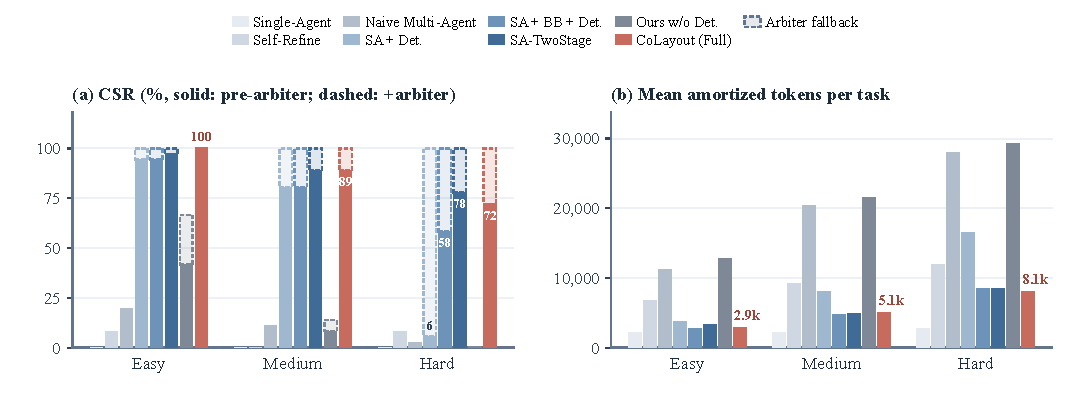
\includegraphics[width=5.45in]{figures/fig2_performance.pdf}
  \caption{Constraint satisfaction and mean amortized tokens by difficulty
  across all \vMethodCount{} methods (\vBriefCount{} briefs $\times$
  \vSeedCount{} seeds; \emph{CoLayout} highlighted in terracotta). In (a), solid
  bars show Pre-CSR and dashed caps mark runs resolved by the Priority Arbiter;
  (b) shows mean amortized tokens per task.}
  \label{fig:performance}
\end{figure*}

\begin{figure*}[t]
  \centering
  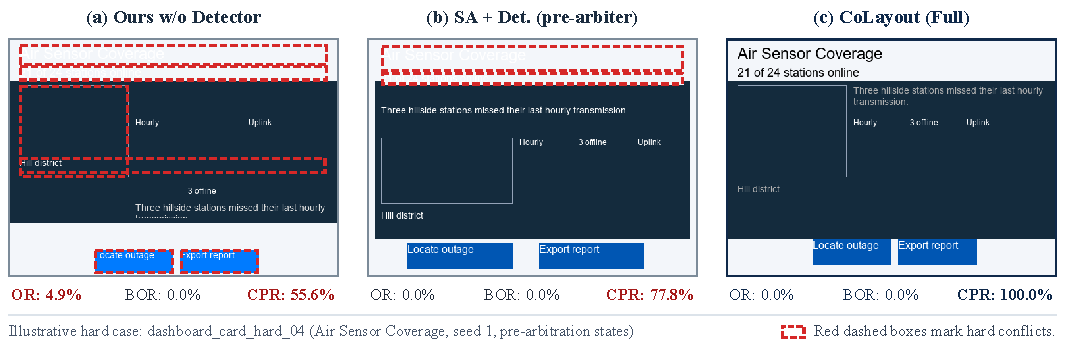
\includegraphics[width=5.45in]{figures/fig3_case_study.pdf}
  \caption{Illustrative hard brief (\emph{\vCaseTitle},
  \vCaseW$\times$\vCaseH~px, seed~\vCaseSeed{}, pre-arbitration states)
  highlighting the two primary drivers. (a)~\emph{Ours w/o Detector} leaves
  \vCaseNDOv{} overlap and \vCaseNDCp{} contrast failures (\vCaseNDTok{}
  tokens); (b)~\emph{SA + Det.}\ clears overlap via deterministic checks but
  still stalls with \vCaseSDCp{} header contrast failures under full-state
  regeneration (\vCaseSDTok{} tokens); (c)~\emph{CoLayout} clears all hard
  checks in \vCaseCoRnd{} rounds (\vCaseCoTok{} tokens, \vCaseCoFit{}
  text-fit).}
  \label{fig:case}
\end{figure*}

\subsection{Protocol, stopping rules, and statistical analysis}
All \vMethodCount{} methods run in one contiguous batch on the pinned snapshot
\texttt{gpt-4o-mini-2024-07-18} (JSON mode, no \texttt{max\_\allowbreak tokens}
cap) across \vSeedCount{} seeds (\vRunsPerMethod{} runs/method, \vRunsTotal{}
completed runs), evaluated under an analysis plan fixed before the full run. We
fix $K=5$: Single-Agent runs one round, Self-Refine and Naive Multi-Agent cap at
five rounds, and the five controlled variants allow initialization plus five
correction rounds (six recorded); all detector-guided methods average
\vRndFull--\vRndSADet{} rounds, well below the cap. Malformed or unknown-key
responses trigger up to two in-round retries without silent drops; if an attempt
still fails validation, the run restarts from scratch with a derived seed (up to
three attempts). With \vResidualFail{} residual failures across
\vFailAttemptsTotal{} retried attempts (highest failure rate \vFailRateMax{} in
SA + Det.), intention-to-treat and complete-case compliance coincide; primary
token means amortize failed attempts. Four controlled contrasts
(Table~\ref{tab:contrasts}) pool all \vSeedCount{} seeds and compute 95\%
brief-clustered percentile bootstrap confidence intervals ($B=20{,}000$,
resampling the \vBriefCount{} briefs or \vHardBriefCount{} hard briefs).

\subsection{Main results and architectural decomposition}
Table~\ref{tab:main}, Table~\ref{tab:contrasts}, and Fig.~\ref{fig:performance}
compare the four steps.

\textbf{Deterministic detection} (\emph{CoLayout} vs.\ \emph{Ours w/o
Detector}) drives the largest compliance and cost gains.
Detector-free baselines rarely converge (\vPreSA--\vPreNaive{} Pre-CSR), and
substituting an LLM critic inside CoLayout's blackboard drops Pre-CSR to
\vPreNoDet{}. Restoring deterministic detection raises Pre-CSR by \vDPreDet{}
overall (hard \vPreFullHard{} vs.\ \vPreNoDetHard{}) while cutting amortized
tokens by \vTokCutDetPct{} (\vTokFull{} vs.\ \vTokNoDet{}).

\textbf{Shared blackboard and partial patches} (\emph{SA + BB + Det.}\ vs.\
\emph{SA + Det.}) are the second major driver. Moving from full-state JSON
regeneration to the versioned blackboard with programmatic copy injection and
partial patches raises Pre-CSR by \vDPreBB{} overall (\vPreSABB{} vs.\
\vPreSADet{}) and \vDPreBBHard{} on hard briefs (\vPreSABBHard{} vs.\
\vPreSADetHard{}), cuts amortized tokens by \vTokCutBBPct{} (\vTokSABB{} vs.\
\vTokSADet{}), and lowers whole-run failure rate from \vFailRateSADet{} to
\vFailRateSABB{}.

\textbf{Sequential initialization} (\emph{SA-TwoStage + BB + Det.}\ vs.\
\emph{SA + BB + Det.}) splits Round~0 into geometry followed by styling while
keeping revision unlocked. Pre-CSR rises from \vPreSABB{} to \vPreTwoStage{}
(\vDPreSeq{} overall; \vDPreSeqHard{} hard), an effect that is directionally
consistent but not statistically significant as both 95\% CIs span zero
(Table~\ref{tab:contrasts}). Amortized token cost stays flat (\vTokTwoStage{}
vs.\ \vTokSABB{}, CI spanning zero), as the extra Round-0 call
(\vCallsTwoStage{} vs.\ \vCallsSABB{} calls) is offset by slightly fewer rounds
(\vRndTwoStage{} vs.\ \vRndSABB{}). Crucially, sequential initialization
significantly reduces Round-0-to-final center displacement by \vDDispSeq{}~px
(Table~\ref{tab:diagnostics}) and box-size drift (mean $|\Delta w|+|\Delta h|$:
\vDwhSABB{} to \vDwhTwoStage{}~px; \vDwhFull{}~px in CoLayout) while raising terminal hard-brief zone adherence (full-box band compliance) from
\vZoneSABB{} to \vZoneTwoStage{} (\vZoneFull{} in CoLayout). This
trades off a significant \vDFitHardSeq{} drop in terminal hard-brief raster
text-fit (\vFitHardTwoStage{} vs.\ \vFitHardSABB{}, 95\% CI \vDFitHardSeqCI{}~pp);
on hard briefs, layout-level joint compliance and 100\% text-fit drops from
\vJointPreHardSABB{} (\emph{SA + BB + Det.}) to \vJointPreHardTwoStage{}
(\emph{SA-TwoStage}) and \vJointPreHardFull{} (\emph{CoLayout}) pre-arbitration
(\vJointFinHardSABB{} vs.\ \vJointFinHardTwoStage{} and \vJointFinHardFull{}
terminally). Across all briefs, \emph{CoLayout} and \emph{SA + BB + Det.}\ tie
at \vJointPreFull{} Pre\&Fit (Table~\ref{tab:main}).

\textbf{Role separation, routing, and field locks} (\emph{CoLayout (Full)} vs.\
\emph{SA-TwoStage + BB + Det.}) show no statistically significant difference in
convergence or cost: Pre-CSR differs by \vDPreLock{} (\vPreFull{} vs.\
\vPreTwoStage{}) and tokens by \vDTokLock{}, with 95\% CIs spanning zero across
Pre-CSR, tokens, displacement (\vDDispLock{}~px), and hard text-fit (identical
at \vFitHardFull{}). Likewise, CoLayout's combined Pre-CSR gain over \emph{SA +
BB + Det.}\ (\vDPreFullBB{}~pp) touches zero. On this benchmark, field locks are
therefore justified by schema-enforced write isolation rather than convergence
speed, complementing the patch-level auditability already provided by the
versioned blackboard.

\begin{table}[t]
\centering
\caption{Repair diagnostics across the four detector-guided methods (108 runs/method). Displacement is mean Round-0-to-final element center shift; Arbiter counts fallback runs; Regressions count contrast-to-geometry (C$\to$G) and geometry-to-contrast (G$\to$C) regressions. Bold marks best.}
\label{tab:diagnostics}
\footnotesize
\setlength{\tabcolsep}{3.0pt}
\resizebox{\columnwidth}{!}{%
\begin{tabular}{@{}lcccc@{}}
\toprule
Diagnostic & SA+Det. & SA+BB+Det. & SA-TwoStage & CoLayout \\
\midrule
Repair displacement (px) $\downarrow$ & 5.07 & 5.00 & 1.66 & \textbf{1.20} \\
Arbiter triggers (/108) $\downarrow$ & 43 & 24 & \textbf{13} & 14 \\
Regressions (C$\to$G / G$\to$C) $\downarrow$ & 0 / 4 & 5 / 3 & \textbf{0 / 0} & \textbf{0 / 0} \\
\bottomrule
\end{tabular}%
}
\end{table}


\subsection{Repair diagnostics and illustrative case}
Under aligned prompts, Round-0 compliance is uniformly low across all four
detector-guided methods (\vRzeroMin--\vRzeroMax{}), showing that sequential
decomposition does not act by solving layouts in Round~0. Instead, separating
geometry from styling cuts Round-0 geometry conflicts from \vRzeroGeomSABB{}
(\emph{SA + BB + Det.}) to \vRzeroGeomTwoStage{} (\emph{SA-TwoStage}) and
\vRzeroGeomFull{} (\emph{CoLayout}) across \vRunsPerMethod{} runs, which is associated with higher revision conversion (share of Round-0 failures
resolved pre-arbitration: \vConvSABB{} to \vConvTwoStage{} and \vConvFull{})
and significantly smaller Round-0-to-final center displacement
(\vDispSABB{}~px to \vDispTwoStage{} and \vDispFull{}~px;
Table~\ref{tab:diagnostics}; \vDDispFullBB{}~px for CoLayout vs.\ SA + BB +
Det.). Priority Arbiter fallback triggers drop correspondingly from
\vArbSADet{} (\emph{SA + Det.}) and \vArbSABB{} (\emph{SA + BB + Det.}) to
\vArbTwoStage{} (\emph{SA-TwoStage}) and \vArbFull{} (\emph{CoLayout}) out of
\vRunsPerMethod{} runs. Finally, unlocked single-agent methods incur
cross-attribute regressions (\vRegCGSABB{} C$\to$G and \vRegGCSABB{} G$\to$C in
\emph{SA + BB + Det.}; \vRegGCSADet{} G$\to$C in \emph{SA + Det.}), whereas both two-stage workflows record \vRegTwoStage{} (\emph{SA-TwoStage}) and
\vRegFull{} (\emph{CoLayout}); in CoLayout, contrast-to-geometry regressions are
ruled out by schema construction rather than prompt adherence. A stricter
offline audit checking worst-case contrast across partially overlapped cards
flags \vStradFlipPreFull/\vRunsPerMethod{} Pre-CSR and
\vStradFlipFinFull/\vRunsPerMethod{} terminal violations in \emph{CoLayout}
(\vStradFlipPreTwoStage{} Pre-CSR, \vStradFlipFinTwoStage{} terminal in
\emph{SA-TwoStage}), versus \vStradFlipPreSABB/\vRunsPerMethod{} Pre-CSR
(\vStradFlipFinSABB{} terminal) in \emph{SA + BB + Det.}\ (strict Pre-CSR
\vStrictPreSABB{}) and \vStradFlipFinSADet{} terminal in \emph{SA + Det.},
leaving all primary conclusions unchanged.

Fig.~\ref{fig:case} illustrates the two primary drivers on \emph{\vCaseTitle}
(seed~\vCaseSeed{}, pre-arbitration): \emph{Ours w/o Detector} leaves
\vCaseNDOv{} overlap (\vCaseNDOR{} OR) and \vCaseNDCp{} contrast failures
(\vCaseNDCPR{} CPR); \emph{SA + Det.}\ resolves overlap (\vCaseSDOR{} OR) and
footer contrast but still stalls on \vCaseSDCp{} header failures (\vCaseSDCPR{}
CPR); and \emph{CoLayout} clears all hard conflicts in \vCaseCoRnd{} rounds
(\vCaseCoTok{} tokens, \vCaseCoFit{} text-fit, zero arbitration).

\section{Discussion, Limitations, and Conclusion}\label{sec:discussion}
\subsection{Trade-offs and design implications}
The controlled ladder exposes a concrete trade-off in sequential initialization:
initializing box dimensions before styling lowers net repair displacement
(\vDispTwoStage{} vs.\ \vDispSABB{}~px; \vDispFull{}~px in \emph{CoLayout}), but without an in-loop text-fit check,
tight initial boxes remain uncorrected during revision, consistent with the
shared \vDFitHardSeq{} hard text-fit drop in \emph{SA-TwoStage} and
\emph{CoLayout} (\vFitHardFull{} vs.\ \vFitHardSABB{}, Table~\ref{tab:main};
all methods color \vCardHardAll{} of hard dark cards). Closing this gap calls for a deterministic text-fit check or cross-role height
expansion requests. Although role separation and field locks show no significant
convergence gain in autonomous runs, explicit write boundaries complement
versioned patch logs in human-in-the-loop co-editing, letting a designer assume one role, pin elements,
or override automated patches on the shared state.

\subsection{Limitations}
This evaluation has four main limitations. All \vRunsTotal{} runs use a single
language model (\texttt{gpt-4o-mini-2024-07-18}), so effect sizes on stronger
reasoning models or open-weight models remain untested. The benchmark spans
\vBriefCount{} synthetic briefs with fixed element inventories and solid
background fills rather than production templates with reflowing copy or
photographic backgrounds. We evaluate deterministic compliance and raster
text-fit without a user study of aesthetic preference or human co-editing
effort. Finally, raster text-fit and partial card-boundary straddling are
audited offline rather than enforced inside the deterministic detector loop.
\ifanonymous
Code, briefs, and raw logs will be released upon acceptance.
\else
Code, briefs, checks, and raw logs are available at
\url{https://github.com/zhouyukai0908/colayout}.
\fi

\subsection{Conclusion}
Across \vMethodCount{} prompt-aligned methods and \vRunsTotal{} multi-seed runs,
our controlled ablation ladder clarifies where gains in shared-state layout
coordination originate: deterministic conflict detection (\vDPreDet{} Pre-CSR,
\vTokCutDetPct{} token reduction) and blackboard partial patching (\vDPreBB{}
Pre-CSR, \vTokCutBBPct{} token reduction) drive convergence and efficiency;
sequential initialization significantly lowers repair displacement and improves
hard-brief zone adherence at a \vDFitHardSeq{} hard-brief text-fit cost; and
role-scoped field locks show no significant convergence difference over an
unlocked two-stage control. Practitioners building LLM layout agents should
prioritize versioned shared-state partial patches and deterministic checking for
convergence and auditability, adding role separation and field locks when
schema-enforced write isolation is required.

\balance
\bibliographystyle{IEEEtran}
\bibliography{refs}
\end{document}
